\documentclass{article}

\usepackage{amsmath}
\usepackage{amssymb}
\usepackage{tikz}

\begin{document}
\begin{enumerate}
\item [1.8.7.1]
  The pullback lemma states that if both squares of the diagram below are pullbacks then the entire rectangle is a pullback.
  In the other direction, it states that if the overall rectangle and right square are pullbacks, the left rectangle is a pullback.
  \begin{center}
    \begin{tikzpicture}
      \node (1) {};
      \node[right of=1,xshift=1cm] (2) {};
      \node[right of=2,xshift=1cm] (3) {};
      \node[below of=1,yshift=-1cm] (4) {};
      \node[right of=4,xshift=1cm] (5) {};
      \node[right of=5,xshift=1cm] (6) {};
      %% Horizontal arrows
      \draw[->] (1) -- (2);
      \draw[->] (2) -- (3);
      \draw[->] (4) -- (5);
      \draw[->] (5) -- (6);
      %% Vertical arrows
      \draw[->] (1) -- (4);
      \draw[->] (3) -- (6);
      \draw[->] (2) -- (5);
    \end{tikzpicture}
  \end{center}

  First, we show that if the squares are pullbacks, the entire rectangle is a pullback.
  That is, we know the following:

  \hfill{}
  \begin{tikzpicture}
    \node (1) {};
    \node[right of=1,xshift=1cm] (2) {};
    \node[below of=1,yshift=-1cm] (4) {};
    \node[right of=4,xshift=1cm] (5) {};
    \node[right of=5,xshift=1cm] (6) {};
    %% Horizontal arrows
    \draw[->] (1) -- node[above]{$f_1$} (2);
    \draw[->] (4) -- node[below] {$f_2$} (5);
    %% Vertical arrows
    \draw[->] (1) -- node[right] {$g_1$} (4);
    \draw[->] (2) -- node[right] {$g_2$} (5);
    %% pullback stuff
    \node[above left of=1,xshift=-1cm,yshift=1cm] (7) {};
    \draw[dashed,->] (7) -- node[above]{$k_1$} (1);
    \draw[->] (7) -- node[above]{$i_1$} (2);
    \draw[->] (7) -- node[left]{$j_1$} (4);  
  \end{tikzpicture}
  \hfill{}
  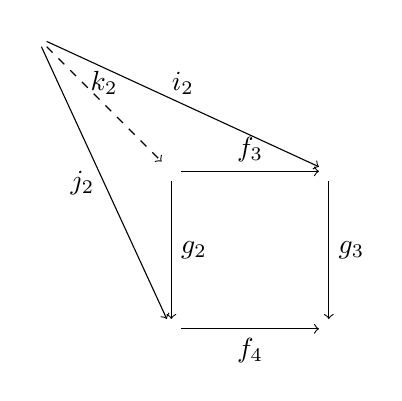
\begin{tikzpicture}
    \node (1) {};
    \node[right of=1,xshift=1cm] (2) {};
    \node[below of=1,yshift=-1cm] (4) {};
    \node[right of=4,xshift=1cm] (5) {};
    %% Horizontal arrows
    \draw[->] (1) -- node[above]{$f_3$}(2);
    \draw[->] (4) -- node[below]{$f_4$}(5);
    %% Vertical arrows
    \draw[->] (1) -- node[right]{$g_2$}(4);
    \draw[->] (2) -- node[right]{$g_3$}(5);
    %% pullback stuff
    \node[above left of=1,xshift=-1cm,yshift=1cm] (7) {};
    \draw[dashed,->] (7) -- node[above]{$k_2$} (1);
    \draw[->] (7) -- node[above]{$i_2$} (2);
    \draw[->] (7) -- node[left]{$j_2$} (4);
  \end{tikzpicture}
  \hfill{}
  
  and want to show that the pair of arrows ($f_1; f_3$), $g$ is a pullback for $(f_2; f_4)$ and $g_1$.

  \begin{center}
    \begin{tikzpicture}
      \node (1) {};
      \node[right of=1,xshift=1cm] (2) {};
      \node[right of=2,xshift=1cm] (3) {};
      \node[below of=1,yshift=-1cm] (4) {};
      \node[right of=4,xshift=1cm] (5) {};
      \node[right of=5,xshift=1cm] (6) {};
      %% Horizontal arrows
      \draw[->] (1) -- node[above] {$f_1; f_3$} (3);
      \draw[->] (4) -- node[below] {$f_2; f_4$} (6);
      %% Vertical arrows
      \draw[->] (1) -- node[right] {$g_1$} (4);
      \draw[->] (3) -- node[right] {$g_3$} (6);
      %% pullback stuff
      \node[above left of=1,xshift=-1cm,yshift=1cm] (7) {};
      \draw[dashed,->] (7) -- node[above]{$k$} (1);
      \draw[->] (7) -- node[above]{$i$} (3);
      \draw[->] (7) -- node[left]{$j$} (4);
    \end{tikzpicture}
  \end{center}

  From the diagram, it is immediately clear that $g_1$ is the pullback arrow of $g_3$ along $(f_2; f_4)$.
  That side of the rectangle is the same as that side of the square.
  More formally, the codomain of $g_1$ is the same as the domain of $(f_2; f_4)$, hence for any arrow $j$ that we could replace $g_1$ with and still have a commutative diagram we can map its domain to $\textbf{dom}(g_1)$ using the unique arrow $k_1$.

  The case for $(f_1; f_3)$ follows because $f_1$ and $f_3$ are the unique pullbacks of $f_2$ and $f_4$ (along $g_2$ and $g_3$), respectively.
  If the arrows are unique then their composition is unique, thus $(f_1; f_3)$ must be the pullback of $(f_2; f_4)$ along $g_3$.

  Next, we show that if the overall rectangle and right square are pullbacks, the left square is a pullback.
  
  That is, we have:
  
  \hfill{}
  \begin{tikzpicture}
    \node (1) {};
    \node[right of=1,xshift=1cm] (2) {};
    \node[right of=2,xshift=1cm] (3) {};
    \node[below of=1,yshift=-1cm] (4) {};
    \node[right of=4,xshift=1cm] (5) {};
    \node[right of=5,xshift=1cm] (6) {};
    %% Horizontal arrows
    \draw[->] (1) -- node[above] {$f_1; f_3$} (3);
    \draw[->] (4) -- node[below] {$f_2; f_4$} (6);
    %% Vertical arrows
    \draw[->] (1) -- node[right] {$g_1$} (4);
    \draw[->] (3) -- node[right] {$g_3$} (6);
    %% pullback stuff
    \node[above left of=1,xshift=-1cm,yshift=1cm] (7) {};
    \draw[dashed,->] (7) -- node[above]{$k$} (1);
    \draw[->] (7) -- node[above]{$i$} (3);
    \draw[->] (7) -- node[left]{$j$} (4);
  \end{tikzpicture}
  \hfill{}
  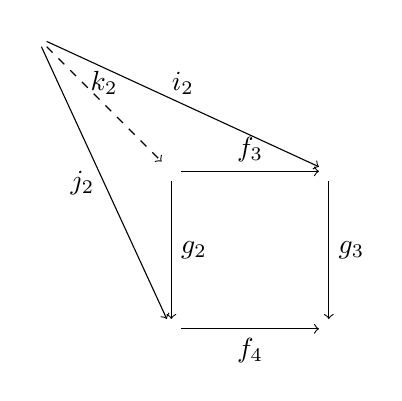
\begin{tikzpicture}
    \node (1) {};
    \node[right of=1,xshift=1cm] (2) {};
    \node[below of=1,yshift=-1cm] (4) {};
    \node[right of=4,xshift=1cm] (5) {};
    %% Horizontal arrows
    \draw[->] (1) -- node[above]{$f_3$}(2);
    \draw[->] (4) -- node[below]{$f_4$}(5);
    %% Vertical arrows
    \draw[->] (1) -- node[right]{$g_2$}(4);
    \draw[->] (2) -- node[right]{$g_3$}(5);
    %% pullback stuff
    \node[above left of=1,xshift=-1cm,yshift=1cm] (7) {};
    \draw[dashed,->] (7) -- node[above]{$k_2$} (1);
    \draw[->] (7) -- node[above]{$i_2$} (2);
    \draw[->] (7) -- node[left]{$j_2$} (4);
  \end{tikzpicture}
  \hfill{}

  and want to show:
  \begin{center}
    \begin{tikzpicture}
      \node (1) {};
      \node[right of=1,xshift=1cm] (2) {};
      \node[below of=1,yshift=-1cm] (4) {};
      \node[right of=4,xshift=1cm] (5) {};
      \node[right of=5,xshift=1cm] (6) {};
      %% Horizontal arrows
      \draw[->] (1) -- node[above]{$f_1$} (2);
      \draw[->] (4) -- node[below] {$f_2$} (5);
      %% Vertical arrows
      \draw[->] (1) -- node[right] {$g_1$} (4);
      \draw[->] (2) -- node[right] {$g_2$} (5);
      %% pullback stuff
      \node[above left of=1,xshift=-1cm,yshift=1cm] (7) {};
      \draw[dashed,->] (7) -- node[above]{$k_1$} (1);
      \draw[->] (7) -- node[above]{$i_1$} (2);
      \draw[->] (7) -- node[left]{$j_1$} (4);  
    \end{tikzpicture}
  \end{center}
  
  Again, we know the arrow $g_1$ is the pullback of $g_2$ along $f_2$.
  This is uniquely determined by the rectangle being a pullback.
  Then to show that $f_1$ is the pullback of $f_2$ along $g_2$, we use the uniqueness of $g_2$ and $f_2$ (which comes from the right square being a pullback).
  Because they are uniquely determined and because the arrow $(f_1; f_2)$ of the overall rectangle is uniquely determined, $f_1$ must be uniquely determined for the left square.

\newpage
\item [1.8.7.2]
  

\newpage
\item [1.8.7.3]
  Given a category where every pair of objects has a product and every pair of arrows with a common codomain has an equalizer, we construct pullbacks for each pair of arrows with a common codomain.
  We begin with our pair of arrows, $f : B \rightarrow D$ and $g : C \rightarrow D$:
  \begin{center}
    \begin{tikzpicture}
      \node (1) {};
      \node[right of=1,xshift=1cm] (2) {$B$};
      \node[below of=1,yshift=-1cm] (3) {$C$};
      \node[right of=3,xshift=1cm] (4) {$D$};

      \draw[->] (2) -- node[right] {$f$} (4);
      \draw[->] (3) -- node[above] {$g$} (4);
    \end{tikzpicture}
  \end{center}
  Because every pair of objects has a product, we can connect the domains of $f$ and $g$ via their product and its projection arrows:
  \begin{center}
    \begin{tikzpicture}
      \node (1) {$B \times C$};
      \node[right of=1,xshift=1cm] (2) {$B$};
      \node[below of=1,yshift=-1cm] (3) {$C$};
      \node[right of=3,xshift=1cm] (4) {};

      \draw[->] (1) -- node[above] {$\pi_2$} (2);
      \draw[->] (1) -- node[left] {$\pi_1$} (3);
    \end{tikzpicture}
  \end{center}
  From here the goal is to connect the diagrams so that they commute.
  However, we do not have that $\pi_1; g = \pi_2; f$; they may not agree on all values.
  But each composition is itself an arrow and we know by assumption that every pair of arrows has an equalizer.
  Therefore we have the equalizer $e$ making $e; \pi_1; g = e; \pi_2; g$ true.
  Moreover this is our pullback.
  For any other arrow from an object $X$ to the domains of $f$ and $g$, we have a unique arrow connecting $X$ to the domain of $e$.
  This is the pullback condition.
  \begin{center}
    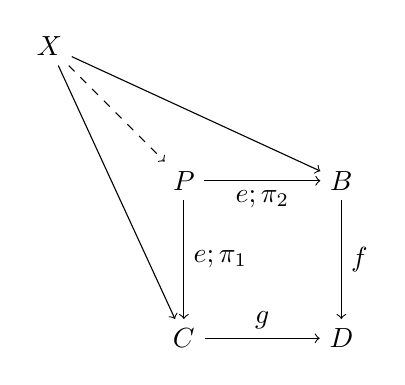
\begin{tikzpicture}
      \node (1) {$P$};
      \node[right of=1,xshift=1cm] (2) {$B$};
      \node[below of=1,yshift=-1cm] (3) {$C$};
      \node[right of=3,xshift=1cm] (4) {$D$};
      \node[above left of=1,xshift=-1cm,yshift=1cm] (5) {$X$};

      \draw[->] (1) -- node[below] {$e; \pi_2$} (2);
      \draw[->] (1) -- node[right] {$e; \pi_1$} (3);
      \draw[->] (2) -- node[right] {$f$} (4);
      \draw[->] (3) -- node[above] {$g$} (4);
      \draw[dashed,->] (5) -- (1);
      \draw[->] (5) -- (2);
      \draw[->] (5) -- (3);
    \end{tikzpicture}
  \end{center}

\newpage
\item [1.8.7.4]
  A pushout of arrows $f : A \rightarrow B$ and $g : A \rightarrow C$ is a pair of arrows $f' : C \rightarrow D$ and $g' : B \rightarrow D$ with a common codomain such that for any other pair of arrows from the domains of $f$ and $g$ to a common codomain $X$ there is a unique arrow $k : D \rightarrow X$ making the following diagram commute.
  \begin{center}
    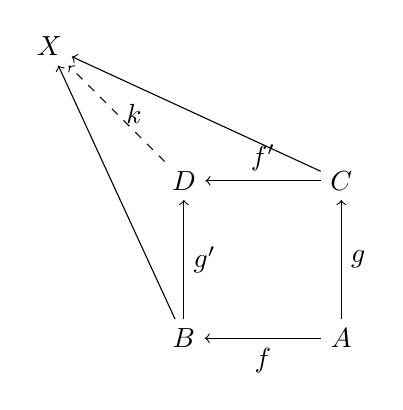
\begin{tikzpicture}
      \node (1) {$D$};
      \node[right of=1,xshift=1cm] (2) {$C$};
      \node[below of=1,yshift=-1cm] (4) {$B$};
      \node[right of=4,xshift=1cm] (5) {$A$};

      \draw[->] (5) -- node[right] {$g$} (2);
      \draw[->] (5) -- node[below] {$f$} (4);

      \draw[->] (2) -- node[above] {$f'$} (1);
      \draw[->] (4) -- node[right] {$g'$} (1);
      %% pullback stuff
      \node[above left of=1,xshift=-1cm,yshift=1cm] (7) {$X$};
      \draw[dashed,->] (1) -- node[right]{$k$} (7);
      \draw[->] (2) -- node[above]{} (7);
      \draw[->] (4) -- node[left]{} (7);
    \end{tikzpicture}
  \end{center}

  This is just a pullback with all arrows reversed.
  Also, in the same way Pierce showed products as pullbacks we can show coproducts as pushouts.
  \begin{center}
    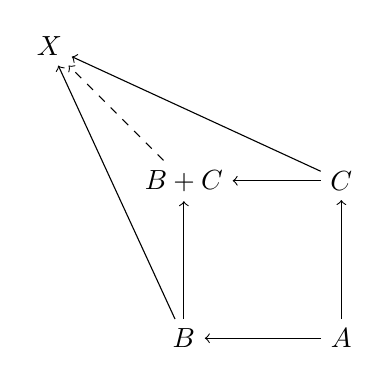
\begin{tikzpicture}
      \node (1) {$B+C$};
      \node[right of=1,xshift=1cm] (2) {$C$};
      \node[below of=1,yshift=-1cm] (4) {$B$};
      \node[right of=4,xshift=1cm] (5) {$A$};

      \draw[->] (5) -- node[right] {} (2);
      \draw[->] (5) -- node[below] {} (4);

      \draw[->] (2) -- node[above] {} (1);
      \draw[->] (4) -- node[right] {} (1);
      %% pullback stuff
      \node[above left of=1,xshift=-1cm,yshift=1cm] (7) {$X$};
      \draw[dashed,->] (1) -- node[right]{} (7);
      \draw[->] (2) -- node[above]{} (7);
      \draw[->] (4) -- node[left]{} (7);
    \end{tikzpicture}
  \end{center}

\end{enumerate}
\end{document}
